\chapter{Teoretická část}

\section{Problém obchodního cestujícího}
Problém obchodního cestujícího patří mezi nejznámější úlohy kombinatorické optimalizace. Jedná se o permutační problém, jehož cílem je nalézt nejkratší uzavřenou cestu, která navštíví množinu zadaných lokalit právě jednou a vrátí se do výchozího bodu.

\subsection{Formální definice problému}
% https://www.cs.vsb.cz/sawa/uti/2025/slides/uti-cz.pdf | 21 slide

Matematicky lze TSP modelovat pomocí teorie grafů. Pro zajištění obecnosti, která zahrnuje i \textbf{asymetrické instance}, definujeme problém na orientovaném grafu. 

Nechť $G = (V, A)$ je úplný orientovaný graf, kde $V = \{v_1, v_2, \dots, v_n\}$ je množina $n$ vrcholů a $A = \{(i, j) : i, j \in V, i \neq j\}$ je množina orientovaných hran. Každé hraně $(i, j)$ je přiřazena nezáporná váha $c_{ij}$, která reprezentuje cenu přesunu (vzdálenost, čas či energii) z vrcholu $i$ do vrcholu $j$. V závislosti na vlastnostech matice cen $\mathbf{C}$ rozlišujeme dvě základní varianty:
\begin{itemize}
    \item \textbf{Symetrické TSP:} Pro všechny dvojice vrcholů platí $c_{ij} = c_{ji}$.
    \item \textbf{Asymetrické TSP:} Existuje alespoň jedna dvojice $(i, j)$ taková, že $c_{ij} \neq c_{ji}$.
\end{itemize}

Cílem je nalézt takovou permutaci $\pi$ indexů $\{1, \dots, n\}$, která minimalizuje celkovou nákladovou funkci:

\begin{equation}
    \min z(\pi) = \sum_{i=1}^{n-1} c_{\pi(i), \pi(i+1)} + c_{\pi(n), \pi(1)}
\end{equation}

Kde jednotlivé členy výrazu reprezentují:
\begin{itemize}
    \item $\pi$ je konkrétní permutace indexů vrcholů z množiny všech přípustných řešení.
    \item $c_{\pi(i), \pi(i+1)}$ vyjadřuje náklady na přesun z vrcholu na $i$-té pozici do vrcholu na pozici $(i+1)$ v daném pořadí $\pi$.
    \item Člen $c_{\pi(n), \pi(1)}$ zajišťuje uzavření cyklu, tedy započtení cesty z posledního navštíveného vrcholu zpět do vrcholu výchozího.
\end{itemize}

Tato uzavřená cesta, která navštíví každý vrchol grafu právě jednou, se v teorii grafů nazývá \textbf{Hamiltonovský cyklus}. V informatice lze vrcholy a hrany reprezentovat maticí sousednosti (vzdáleností) $\mathbf{C} = [c_{ij}]_{n \times n}$, kde jednotlivé prvky představují váhy hran mezi dvojicemi vrcholů $v_i$ a $v_j$. Tato reprezentace umožňuje efektivní algoritmické zpracování stavového prostoru problému a je základem pro většinu implementací heuristických i exaktních algoritmů.

\begin{equation}
\label{eq:general_cost_matrix}
C = 
\begin{pmatrix}
v_{11} & v_{12} & \cdots & v_{1n} \\
v_{21} & v_{22} & \cdots & v_{2n} \\
\vdots & \vdots & \ddots & \vdots \\
v_{n1} & v_{n2} & \cdots & v_{nn}
\end{pmatrix}
\end{equation}

\subsection{Ilustrace problému a řešení}

Pro lepší pochopení podstaty TSP je vhodné interpretovat instanci graficky. Na obrázcích je znázorněn rozdíl mezi neoptimalizovaným stavem na obrázku \ref{fig:neoptimalni_tsp} a nalezeným přípustným řešením po aplikaci optimalizačního algoritmu, které je zobrazeno na obrázku \ref{fig:optimalni_tsp}.

\begin{itemize}
    \item \textbf{Neoptimalizovaná instance:} Představuje náhodné nebo abecední seřazení lokalit, které má obchodní cestující navštívit. V grafickém znázornění je patrný vizuální chaos a velké množství křížících se hran. Celková délka takové trasy je z logistického hlediska neefektivní a představuje horní odhad nákladů.
    \item \textbf{Optimalizovaná instance:} Zobrazuje výsledek hledání Hamiltonovské kružnice s minimální (nebo blízkou minimální) celkovou délkou. V euklidovském prostoru je typickým znakem optima absence křížení hran a plynulé navazování cesty mezi geograficky blízkými uzly.
\end{itemize}

\begin{figure}[H]
  \centering
  \begin{minipage}[b]{0.4\textwidth}
    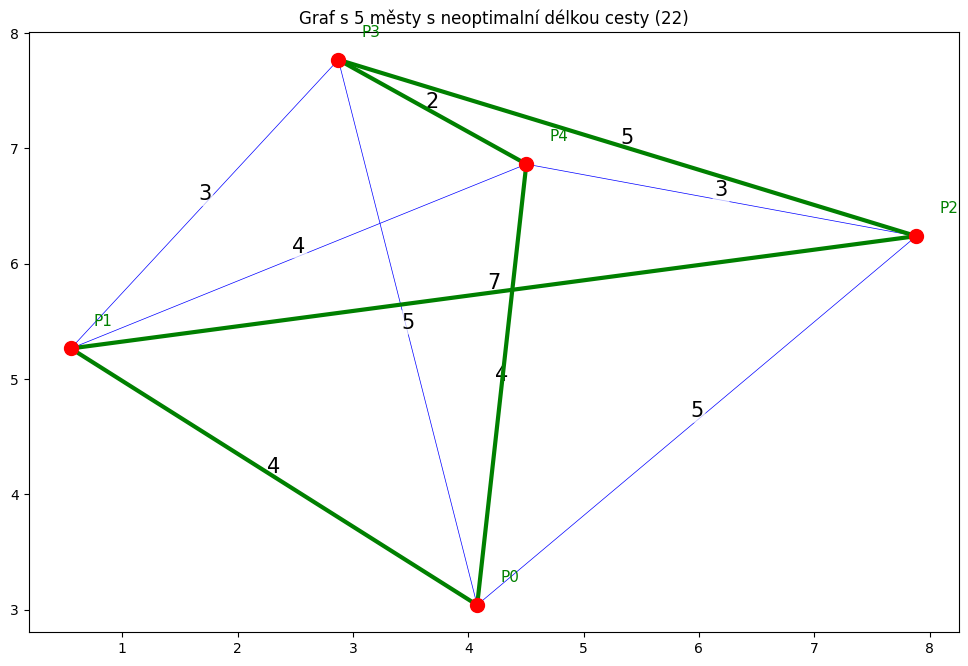
\includegraphics[width=\textwidth]{Figures/neoptimalni_tsp.png}
    \caption{Neoptimální instance}
    \label{fig:neoptimalni_tsp}
  \end{minipage}
  \hfill
  \begin{minipage}[b]{0.4\textwidth}
    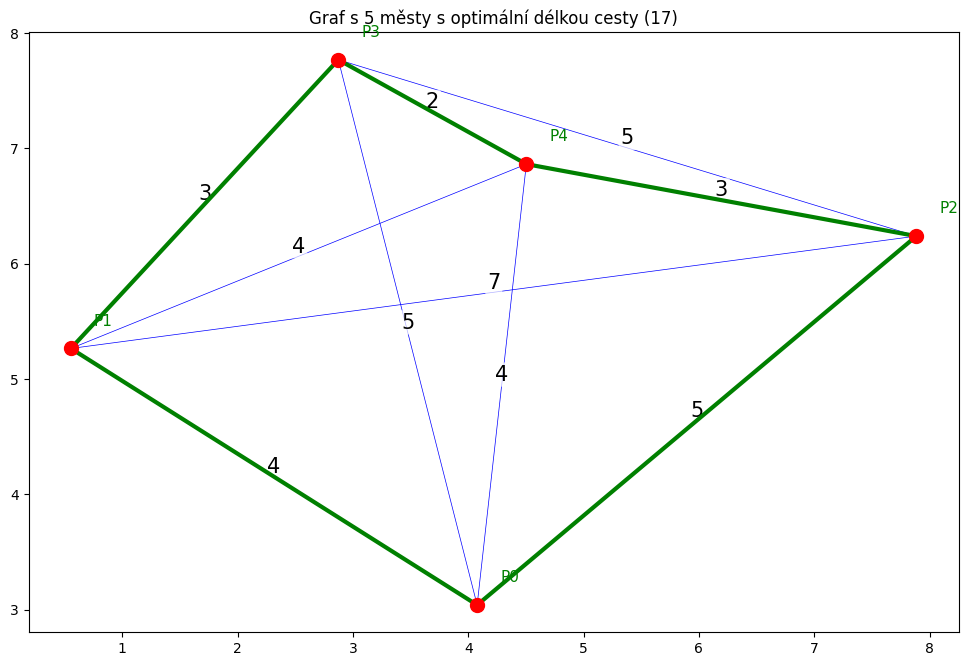
\includegraphics[width=\textwidth]{Figures/optimalni_tsp.png}
    \caption{Optimální instance}
    \label{fig:optimalni_tsp}
  \end{minipage}
\end{figure}

% TODO reference na TSPLIB dokumentaci
\subsection{Typy TSP}
Jak bylo definováno v předchozí části, základním datovým vstupem pro řešení problému je matice vzdáleností $\mathbf{C}$, kde prvek $c_{ij}$ reprezentuje ohodnocení hrany mezi uzly $v_i$ a $v_j$. V závislosti na vnitřních vlastnostech této matice a charakteru reálného prostředí, které má generátor simulovat, rozlišujeme následující varianty:

\begin{itemize}
    \item \textbf{Symetrický TSP (STSP):} Tato varianta předpokládá, že matice $\mathbf{C}$ je symetrická podle hlavní diagonály, tedy platí $c_{ij} = c_{ji}$ pro všechna $i, j \in V$. V praxi to znamená, že náklady na cestu z bodu $A$ do bodu $B$ jsou identické jako v opačném směru. Tento model je typický pro euklidovské instance (např. typ \texttt{EUC\_2D} v TSPLIB), kde je vzdálenost počítána jako norma v rovině.
    
    \item \textbf{Asymetrický TSP (ATSP):} Zde podmínka symetrie neplatí a v matici existuje alespoň jeden pár indexů, pro který $c_{ij} \neq c_{ji}$. Pro náš generátor využívající mapová API je tato varianta klíčová, neboť v reálné silniční síti jsou náklady na přesun ovlivněny jednosměrnými ulicemi, dálničními nájezdy nebo výškovým profilem trasy.
    
    \item \textbf{Metrický TSP (trojúhelníková nerovnost):} Jedná se o typ, kde prvky matice splňují trojúhelníkovou nerovnost: $c_{ij} \leq c_{ik} + c_{kj}$ pro libovolnou trojici vrcholů. U reálných silničních dat tato vlastnost závisí na volbě nákladové funkce a konkrétních omezeních dopravy; nelze ji proto obecně předpokládat pro všechny typy výstupů mapových služeb.
    
    \item \textbf{Dynamický TSP:} Na rozdíl od statických matic v TSPLIB, v této variantě je $c_{ij}$ funkcí času $c_{ij}(t)$. To umožňuje reflektovat proměnlivou dopravní situaci (např. dopravní špičky zjištěné přes API).
\end{itemize}


% TODO citace jančara a sawy
\subsection{NP-úplnost a výpočetní složitost}
Z hlediska teorie složitosti je nezbytné u TSP rozlišovat mezi jeho optimalizační a rozhodovací variantou. Optimalizační úloha, tedy hledání Hamiltonovské kružnice s minimálním součtem vah hran, spadá do třídy \textbf{NP-těžkých} (NP-hard) problémů. To znamená, že pro ni neexistuje známý algoritmus s polynomem omezenou časovou složitostí, pokud neplatí $P = NP$.%\cite{sawa}.

Rozhodovací verze TSP (označovaná jako \textit{TSP decision problem}) se ptá, zda v daném grafu $G$ existuje Hamiltonovská kružnice s celkovou vahou $c \leq k$ pro zadanou konstantu $k$. Tato varianta patří mezi \textbf{NP-úplné} problémy. Její náročnost lze dokázat polynomiální redukcí z problému Hamiltonovské kružnice (HC), který je jedním z klasických NP-úplných problémů %\cite{jancar, sawa}.
Výpočetní náročnost je dána explozivním růstem stavového prostoru. 

Pro symetrický problém s $n$ vrcholy existuje celkem
\begin{equation}
    \frac{(n-1)!}{2}
\end{equation}
možných přípustných řešení (Hamiltonovských kružnic). V případě asymetrického problému, který je klíčový pro náš generátor, je počet možných cest $(n-1)!$. %\cite{sawa}
Tento faktoriální růst způsobuje, že i pro relativně malé instance (např. $n=20$) je nalezení globálního optima metodou hrubé síly v reálném čase neproveditelné. Zatímco ověření kandidátního řešení (zda je cesta Hamiltonovská a zda její váha nepřekračuje $k$) je řešitelné v polynomiálním čase, samotné nalezení optima vyžaduje nasazení pokročilých heuristik nebo aproximačních algoritmů, kterým se věnuje kapitola \ref{subsection:BIA}.


\section{Stanovení vah hran v reálných sítích}
V klasických formulacích TSP se předpokládá, že váhy hran jsou již definovány. V rámci této práce, která se zaměřuje na generování instancí z reálných geografických dat, je však klíčovým krokem výpočet nejkratších cest mezi každou dvojicí lokalit v grafu silniční sítě. Tento proces předchází samotnému řešení TSP a využívá algoritmy pro hledání nejkratší cesty mezi dvěma body (\textit{Point-to-Point Shortest Path}).

\subsection{Dijkstrův algoritmus}
Dijkstrův algoritmus je deterministický algoritmus pro hledání nejkratších cest z jednoho zdrojového uzlu do všech ostatních v grafu s nezápornými vahami hran. Algoritmus udržuje množinu navštívených uzlů a pro každý uzel si pamatuje aktuální nejkratší nalezenou cestu. V každém kroku expanduje uzel s minimální dosaženou vzdáleností. Mapové služby využívají Dijkstru (často v kombinaci s technikou \textit{Contraction Hierarchies}) k výpočtu jednotlivých prvků $c_{ij}$ matice vzdáleností.


\subsection{Algoritmus A*}
A* je rozšíření Dijkstrova algoritmu, které využívá heuristickou funkci k urychlení výpočtu.
\begin{itemize}
    \item \textbf{Heuristika:} Zatímco Dijkstra prohledává graf všemi směry, A* upřednostňuje uzly, které leží směrem k cíli (např. na základě euklidovské vzdálenosti).

\begin{equation}
\label{eq:a_star}
f(n) = g(n) + h(n)
\end{equation}
Kde:
\begin{itemize}
    \item $g(n)$ představuje skutečnou cenu z počátečního uzlu do uzlu $n$.
    \item $h(n)$ je odhad ceny cesty z uzlu $n$ do cílového uzlu (můžeme si to představit jako vzdušnou vzdálenost).
\item $f(n)$ je celková ohodnocovací funkce určující prioritu uzlu v rámci prohledávání. Algoritmus pracuje na principu minimalizace této funkce, kdy v každém kroku expanduje uzel $n$ s nejnižší vypočtenou hodnotou $f(n)$, což zajišťuje efektivní směrování výpočtu k cílovému bodu.
\end{itemize}
    \item \textbf{Význam:} V kontextu této práce je A* klíčový pro pochopení, jak routovací enginy dosahují uspokojivých výsledků i nad rozsáhlými mapovými podklady.
\end{itemize}





\section{Metody řešení TSP} %\cite{ti_jancar}
Vzhledem k prokázané NP-těžkosti problému je volba metody řešení vždy kompromisem mezi výpočetním časem a kvalitou nalezeného řešení. Metody lze kategorizovat do čtyř hlavních skupin.

\subsection{Přesné metody}
Tyto algoritmy garantují nalezení globálního optima, avšak jejich časová složitost je v nejhorším případě exponenciální.
\begin{itemize}
\item \textbf{Brute Force:} 
    Tento naivní přístup spočívá v systematickém generování všech přípustných řešení, tedy všech možných Hamiltonovských kružnic v grafu. Algoritmus vypočítá délku každé takové trasy a vybere tu s minimální hodnotou.
    
    \textit{Složitost a limity:} Časová složitost $O(n!)$ představuje jeden z nejrychleji rostoucích typů složitosti. Zatímco pro $n=10$ je počet kombinací řádově v milionech, což moderní procesory zvládnou v přijatelném čase, pro $n=20$ již počet kombinací přesahuje snesitelný počet kombinací, což by vyžadovalo roky výpočetního času. Metoda je tedy využitelná pouze pro verifikaci optimálních řešení u triviálních instancí nebo jako základ pro testování heuristik %\cite{sawa2025}.

    \item \textbf{Branch and Bound:} 
    Jedná se o metodu prohledávání stavového prostoru, která na rozdíl od hrubé síly neprochází všechny kombinace, ale ořezává ty části stromu řešení, které prokazatelně nemohou vést k optimu. Algoritmus využívá dvě základní operace:
    \begin{enumerate}
        \item \textbf{Větvení (Branching):} Rozdělení aktuálního problému na menší podproblémy (např. zahrnutí nebo vyloučení konkrétní hrany $e_{ij}$ z trasy).
        \item \textbf{Určování mezí (Bounding):} Pro každý uzel ve stromu výpočtu se určí dolní mez (lower bound) ceny řešení. Tato mez se často získává pomocí relaxace problému (např. řešením přiřazovacího problému nebo výpočtem minimální kostry grafu).
    \end{enumerate}
    
    Pokud je vypočtená dolní mez určité větve vyšší než cena doposud nejlepšího nalezeného řešení (\textit{upper bound}), je celá tato větev z dalšího prohledávání vyřazena. 
    
    \textit{Výhody:} Garantuje nalezení globálního optima a u mnoha reálných instancí je řádově rychlejší než Held-Karpův algoritmus, protože nemusí prohledávat celý stavový prostor.
    
    \textit{Nevýhody:} V nejhorším případě (např. u špatně zvolené relaxace pro výpočet mezí) může složitost stále degradovat na exponenciální, což limituje jeho použití pro rozsáhlé logistické sítě %\cite{reinelt1994}.
    
\item \textbf{Dynamické programování (Bellman-Held-Karpův algoritmus):} 
Tento přístup využívá principu optimality, kdy optimální řešení celého problému lze sestavit z optimálních řešení jeho podproblémů. Na rozdíl od metod typu Branch and Bound, které prohledávají větve stromu a ořezávají je na základě mezí, Held-Karpův algoritmus systematicky buduje tabulku výsledků pro všechny možné podmnožiny měst.

\textit{Princip:} Nechť $S \subseteq V \setminus \{v_1\}$ je podmnožina měst a $g(v_i, S)$ je délka nejkratší cesty začínající v počátečním městě $v_1$, procházející všemi městy v $S$ právě jednou a končící v městě $v_i$. Algoritmus rekurzivně vypočítává hodnoty $g$ pro rostoucí velikost množiny $S$, přičemž využívá již vypočtené hodnoty uložené v paměti.

\textit{Složitost a limity:} Časová složitost je pevně dána vztahem $O(n^2 2^n)$, což je výrazně lepší než faktoriální složitost hrubé síly $O(n!)$, ale stále exponenciální. Hlavním kritickým bodem pro implementaci v rámci našeho generátoru je však \textbf{prostorová (paměťová) náročnost} $O(n 2^n)$, která je způsobena nutností uchovávat tabulku mezivýsledků. V praxi to znamená, že zatímco Branch and Bound může u "šťastných" instancí vyřešit i 40-100 měst, Held-Karp naráží na limity RAM už u instancí kolem $n \approx 25$ až $30$ %\cite{reinelt1994}.

\textit{Výhody:} Garantuje nalezení optima a jeho časový průběh je deterministický (není závislý na kvalitě prořezávání jako u Branch and Bound).

\textit{Nevýhody:} Extrémní nároky na operační paměť a nepoužitelnost pro rozsáhlé logistické sítě, které jsou cílem této práce.
\end{itemize}

\subsection{Heuristiky a lokální optimalizace}
Lokální optimalizace (označované také jako metody lokálního prohledávání) pracují na principu iterativního vylepšování již existujícího přípustného řešení. Cílem je najít v definovaném okolí aktuální trasy takovou změnu, která sníží celkovou cenu .

\begin{itemize}
    \item \textbf{Algoritmy $k$-opt (2-opt a 3-opt):} Číslo $k$ definuje počet hran aktuálního cyklu, které jsou v jednom kroku odstraněny a následně nahrazeny jinou kombinací hran tak, aby byla zachována integrita Hamiltonovské kružnice.
    \begin{itemize}
    \item \textbf{Princip 2-opt (záměna dvou hran):} 
    Představme si aktuální trasu jako uzavřený řetězec. Algoritmus vybere dvě hrany, které nesousedí (tedy nemají společný uzel). Tyto dvě hrany odstraní, čímž se trasa rozpadne na dvě samostatné cesty. Aby vznikla nová souvislá Hamiltonovská kružnice, musí algoritmus tyto dva úseky znovu propojit, ale v jiném pořadí.
    Pokud byla původní cesta $[A \to B \to \dots \to C \to D]$, po odstranění hran $(A,B)$ a $(C,D)$ a následném křížovém propojení vznikne trasa $[A \to C \to \dots \to B \to D]$. 
    
    
    \textit{Geometrický význam:} Pokud se původní dvě hrany křížily, tato operace křížení odstraní. V eukleidovských instancích vede odstranění křížení typicky ke zkrácení trasy; nejde však o univerzální tvrzení pro libovolnou matici nákladů.
        \item \textbf{3-opt:} Tento přístup odstraňuje tři hrany současně, což umožňuje provádět mnohem komplexnější úpravy cesty (včetně přehození celých úseků trasy). Zatímco 2-opt dokáže najít pouze lokální optimum v rámci jednoduchých prohozů, 3-opt prohledává širší okolí řešení, což zvyšuje šanci na nalezení kvalitnější trasy, ovšem za cenu vyšší výpočetní náročnosti ($O(n^3)$ oproti $O(n^2)$ u 2-opt).
\end{itemize}
    \item \textbf{Lin-Kernighan (LK):} Algoritmus Lin-Kernighan je v podstatě zobecněním $k$-opt přístupu, kde hodnota $k$ není předem fixně stanovena. Algoritmus v každém kroku adaptivně rozhoduje, kolik hran je vhodné zaměnit, a to na základě potenciálního zlepšení nákladové funkce. Díky této flexibilitě dokáže LK efektivně opustit lokální minima, ve kterých by se standardní 2-opt nebo 3-opt algoritmy zastavily. V praxi se často používá k dosažení řešení, která jsou velmi blízko optimu i pro instance s tisíci uzly.
\end{itemize}

\subsection{Metaheuristiky a biologicky inspirované algoritmy}
\label{subsection:BIA}
Vzhledem k výpočetní náročnosti přesných metod se pro rozsáhlé instance moderní logistiky využívají metaheuristiky. Tyto algoritmy nehledají globální optimum s absolutní jistotou, ale zaměřují se na nalezení dostatečně kvalitního řešení v akceptovatelném čase. Klíčovou vlastností těchto metod je schopnost unikat z lokálních optim pomocí mechanismů inspirovaných přírodou.

\begin{itemize}
    \item \textbf{Genetické algoritmy (GA):} Tato technika simuluje proces přírodního výběru a evoluce. Místo jednoho řešení pracuje s celou populací (množinou tras). Jednotlivci jsou podrobováni operacím selekce (výběr nejlepších), křížení (výměna úseků tras mezi „rodiči“) a mutace (náhodná změna trasy). Pro TSP je nutné využívat specifické operátory jako \textit{Order Crossover} (OX) nebo \textit{Edge Recombination Crossover} (ERX), které zaručují, že vzniklí potomci budou stále platnými permutacemi bez chybějících či duplicitních měst.
    
    \item \textbf{Mravenčí kolonie (Ant Colony Optimization - ACO):} Algoritmus je inspirován chováním mravenců při hledání nejkratší cesty k potravě. Umělí agenti (mravenci) konstruují řešení tak, že se pohybují po hranách grafu, přičemž jejich volba je ovlivněna množstvím feromonu na hraně a její délkou. Hrany, které jsou součástí kratších cest, získávají v iteracích více feromonu. Důležitým mechanismem je vypařování feromonu v čase, což zabraňuje příliš rychlé konvergenci do lokálního optima a umožňuje prohledávat nové oblasti stavového prostoru.
    
    \item \textbf{Simulované žíhání (Simulated Annealing - SA):} Metoda vychází z analogie k ochlazování kovů v metalurgii. Algoritmus začíná při vysoké „teplotě“, kdy s vysokou pravděpodobností přijímá i horší řešení než to stávající, což mu umožňuje uniknout z mělkých lokálních minim. S postupným ochlazováním tato pravděpodobnost klesá a algoritmus se začíná chovat spíše jako lokální optimalizace, která konverguje k finálnímu řešení.
    
    \item \textbf{Particle Swarm Optimization - PSO:} Původně spojitý algoritmus simulující pohyb hejna ptáků či ryb. V diskrétní verzi pro TSP (DPSO) každá částice představuje konkrétní trasu a její „pohyb“ je definován jako aplikace posloupnosti swap operací, které ji přibližují k jejímu dosavadnímu nejlepšímu řešení a zároveň k nejlepšímu řešení celého hejna.
    
\item \textbf{Rat Swarm Optimizer (RSO):} Biologicky inspirovaný algoritmus, který simuluje inteligentní chování potkanů v hejnu během procesu lovu. Algoritmus je strukturálně rozdělen do dvou klíčových fází:
\begin{itemize}
    \item \textbf{Fáze pronásledování (Chasing):} V této fázi se potkani pohybují směrem k lídrovi (nejlepšímu dosud nalezenému řešení). Matematicky je tento pohyb definován tak, aby agenti efektivně prohledávali okolí a balancovali mezi náhodným pohybem a následováním nejúspěšnějšího jedince. To umožňuje algoritmu pokrýt širokou oblast stavového prostoru a vyhnout se uvíznutí v lokálním optimu.
    \item \textbf{Fáze boje (Fighting):} V kontextu TSP to znamená jemné ladění trasy v blízkosti nejlepšího nalezeného řešení. Tato fáze je zodpovědná za rychlou konvergenci algoritmu k finálnímu výsledku.
\end{itemize}
Díky této kombinaci globálního prohledávání a lokálního zpřesňování dosahuje RSO dobrých výsledků i na komplexních instancích.
\end{itemize}


\subsection{Aproximační a konstruktivní algoritmy}
Na rozdíl od běžných heuristik poskytují aproximační algoritmy pevnou matematickou garanci, která definuje maximální možnou odchylku nalezeného řešení od globálního optima. %\cite{ti_sawa}.
Tyto algoritmy jsou klíčové pro pochopení mezí výpočetní složitosti u metrických variant TSP.

\begin{itemize}
    \item \textbf{Nearest Neighbour:} 
    Tento algoritmus reprezentuje tzv. greedy přístup. Začíná v náhodně zvoleném uzlu a v každém dalším kroku se přesune do nejbližšího dosud nenavštíveného uzlu. Po navštívení všech měst se algoritmus vrátí do výchozího bodu. 
    
    \textit{Vlastnosti:} Je extrémně rychlý s časovou složitostí $O(n^2)$, avšak postrádá globální nadhled. Často se stává, že v závěru algoritmu zbývají uzly, které jsou od sebe velmi vzdálené, což vede k vytvoření neúměrně dlouhé závěrečné hrany.
    
    \item \textbf{Algoritmus založený na minimální kostře (MST):} 
    Pro instance splňující trojúhelníkovou nerovnost využívá tento přístup vlastností minimální kostry grafu. 
    
    \textit{Princip:} Nejdříve se sestrojí MST daného grafu. Následně se všechny hrany této kostry zdvojí, čímž vznikne multigraf, ve kterém lze nalézt Eulerovský tah. Tento tah se následně transformuje na Hamiltonovskou kružnici pomocí zkratek, kdy vynecháváme již navštívené uzly a propojujeme přímo uzel předchozí s následujícím nenavštíveným. Tím využijeme vlastnost trojúhelníkové nerovnosti a získané řešení má délku nejvýše dvojnásobku optima.

    \item \textbf{Christofidesův algoritmus:} 
    Aktuálně jeden z nejlepších známých aproximačních algoritmů pro metrické TSP, který vylepšuje metodu založenou na MST \cite{ti_sawa}.
    
    \textit{Princip:} Místo zdvojení všech hran kostry algoritmus identifikuje vrcholy s lichým stupněm v MST a nad nimi sestrojí minimální perfektní párování (Minimum Weight Perfect Matching). Výsledný graf je eulerovský a po aplikaci zkratek získáme Hamiltonovskou kružnici.
    
    \textit{Garance:} Tento přístup poskytuje teoretickou garanci $1,5$-aproximace ($L \leq 1,5 \cdot L^*$). \cite{ti_jancar, ti_sawa}.
\end{itemize}




\subsection{Stručné porovnání přístupů}
\begin{table}[h]
\centering
\renewcommand{\arraystretch}{1.3} % Pro lepší čitelnost řádků
\begin{tabular}{|p{3cm}|p{4.5cm}|p{4.5cm}|}
\hline
\textbf{Typ metody} & \textbf{Výhody} & \textbf{Nevýhody} \\ \hline
\textbf{Přesné metody} & Garantují nalezení globálního optima. & Exponenciální časová a prostorová složitost. \\ \hline
\textbf{Aproximační algoritmy} & Teoreticky garantovaná odchylka od optima, rychlost výpočtu. & Omezeno převážně na metrické instance (trojúhelníková nerovnost). \\ \hline
\textbf{Heuristiky} & Extrémně vysoká rychlost, jednoduchá implementace. & Riziko uvíznutí v lokálním optimu, nízká kvalita u velkých instancí. \\ \hline
\textbf{Bio-inspirované algoritmy} & Robustnost, schopnost unikat z lokálních optim, dobrý poměr kvalita/čas. & Nutnost ladění parametrů, stochastický charakter (výsledek se může lišit). \\ \hline
\end{tabular}
\caption{Porovnání metod řešení TSP z hlediska praktického využití}
\label{tab:srovnani_metod}
\end{table}

\section{Datové sady a zdroje geografických dat}
Pro objektivní testování a porovnávání výkonnosti algoritmů jsou nezbytné standardizované datové sady, benchmarky. V kontextu této práce je však nutné rozlišovat mezi historickými syntetickými daty a moderními instancemi založenými na reálné dopravní infrastruktuře.

\subsection{Knihovny TSPLIB a TSPLIB95}
Knihovna TSPLIB, představuje standard pro testování algoritmů řešících TSP. Obsahuje široké spektrum instancí, od vrtání plošných spojů až po simulace měst cesta.
\begin{itemize}
    \item \textbf{Formát .tsp:} Strukturovaný textový soubor obsahující metadata (název, typ metriky, dimenze) a samotná data, která jsou definována buď souřadnicemi uzlů (pro výpočet euklidovské vzdálenosti), nebo explicitní maticí vzdáleností cesta.
    \item \textbf{Formát .opt.tour:} Referenční soubor obsahující sekvenci indexů vrcholů, která tvoří prokazatelně optimální řešení dané instance.
\end{itemize}

\subsection{Limity stávajících benchmarků}
Ačkoliv je TSPLIB stále celosvětově uznávaná, její instance jsou často několik desetiletí staré a neodrážejí dynamickou povahu moderní logistiky. Hlavní nedostatky, které se tato práce snaží eliminovat, zahrnují:
\begin{itemize}
    \item \textbf{Geometrické zjednodušení:} Většina instancí (např. typ \texttt{EUC\_2D}) předpokládá, že nejkratší cesta mezi body je přímka, což v reálném světě neplatí.
    \item \textbf{Absence asymetrie:} Reálná silniční síť obsahuje jednosměrné komunikace a výškové úrovně, což vyžaduje asymetrický přístup (ATSP), zatímco staré sady jsou dominantně symetrické.
    \item \textbf{Statický charakter:} Historická data neumožňují zohlednit aktuální dopravní situaci či uzavírky.
\end{itemize}

\section{Technologické podklady pro generování instancí}
Aby bylo možné generovat instance odpovídající moderním požadavkům, využívá práce API geolokačních a mapových služeb.

\subsection{Geografický podklad: OpenStreetMap (OSM)}
OSM představuje kolaborativní projekt poskytující volně dostupná geografická data. Pro vyvíjený generátor slouží jako primární zdroj topologie silniční sítě, nad kterou jsou počítány reálné vzdálenosti.

\subsection{Routovací engine: OpenRouteService a OSRM}
Pro transformaci geografických souřadnic do matice vzdáleností jsou využívány následující routovací služby:
\begin{itemize}
    \item \textbf{OpenRouteService:} Primární síťová služba použitá v aplikaci pro výpočet matic, geokódování a získání detailů trasy
    \item \textbf{OSRM (Open Source Routing Machine):} Lokálně provozovaný náhradní zdroj pro výpočet matic a tras při nedostupnosti primární služby
\end{itemize}

\subsection{Metodika výpočtu matice vzdáleností}
Výpočet matice vzdáleností představuje kritický prvek přípravy TSP instance. Z hlediska grafové teorie jde o úlohu hledání nejkratších cest mezi všemi dvojicemi vrcholů. Zatímco v teoretických modelech se vzdálenost často počítá jako euklidovská metrika, v reálných logistických systémech je nutné pracovat s váženým orientovaným grafem silniční sítě.

Základem výpočtu v moderních routovacích enginech je Dijkstrův algoritmus, případně jeho vylepšená varianta A*. Vzhledem k obrovskému rozsahu celosvětové silniční sítě (OpenStreetMap obsahuje stovky milionů hran) by však standardní výpočet trval neúnosně dlouho. Proto se využívají pokročilé techniky předzpracování grafu:

\begin{itemize}
    \item \textbf{Contraction Hierarchies (CH):} Tato technika vytváří hierarchickou strukturu grafu, kde jsou méně významné vrcholy (např. v obytných zónách) postupně „stahovány“ do zkratek mezi významnějšími uzly. Výpočet cesty se pak redukuje na prohledávání výrazně menšího počtu hran v hierarchii.
    \item \textbf{Many-to-Many Routing:} Routovací API jsou optimalizována tak, aby nepočítala každou trasu izolovaně. Využívají faktu, že cesty z jednoho zdroje k více cílům často sdílejí stejné segmenty (podstromy nejkratších cest), což dramaticky snižuje počet operací nad prioritní frontou algoritmu.
\end{itemize}

Výsledkem je matice $C$ o rozměrech $n \times n$, kde prvek $c_{ij}$ odpovídá váze nejkratší cesty z uzlu $i$ do uzlu $j$ v grafu silniční sítě.

\subsection{Optimalizační kritéria v moderní logistice}
V klasickém TSP je cílem minimalizace celkové ujeté vzdálenosti. Moderní logistika a systémy pro řízení vozového parku však vyžadují flexibilitu při volbě optimalizačního kritéria. Výběr metriky zásadně ovlivňuje strukturu výsledné matice vzdáleností i podobu optimální trasy.

\begin{enumerate}
    \item \textbf{Metrika nejkratší trasy:} Minimalizuje fyzický počet ujetých kilometrů. Tato varianta je vhodná pro snižování opotřebení vozidel, ale v reálném provozu často vede k nevhodným trasám (např. průjezdy centry měst nebo nekvalitními silnicemi nižších tříd), které jsou časově náročné.
    \item \textbf{Metrika nejrychlejší trasy:} Minimalizuje celkový čas strávený na cestě. Tato metrika zohledňuje rychlostní limity na jednotlivých úsecích, typy komunikací (dálnice vs. místní komunikace) a případně i historickou či aktuální plynulost dopravy. V asymetrickém TSP je tato metrika dominantní, neboť zohledňuje i zdržení na světelných křižovatkách či zákazy odbočení.
\end{enumerate}

Rozdíl mezi těmito kritérii je patrný zejména u velkých instancí, kde nejrychlejší trasa může být výrazně delší než ta nejkratší, ale díky využití dálniční sítě může ušetřit čas. Navrhovaný generátor proto musí umožňovat volbu mezi těmito váhovými funkcemi, aby reflektoval potřeby reálného plánování, kde je prioritou často včasné doručení zásilky na úkor mírného navýšení nájezdu kilometrů.
\endinput